\section{Тест производительности}
\par Для теста производительности я скомпилировал программу с ключом оптимизации -o2, а время работы программы замерял с помощью утилиты time.

Для начала я измерил время создания базы для поиска с разным размером входных файлов. Я сделал 4 замеряя для музыкальных файлов общим размером примерно 100мб, 400мб, 800мб и 1600мб. Вот результаты:

\begin{itemize}
	\item 100mb -- 0m15.153s
	\item 400mb -- 1m10.778s
	\item 800mb -- 2m26.658s
	\item 1600mb -- 4m43.212s
\end{itemize}

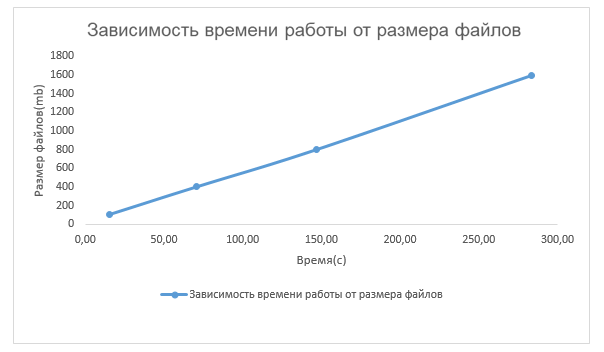
\includegraphics{sizeF_time.png}

Отсюда видно, что сложность создания базы чуть больше чем линейная.

График размеров полученных баз при этих же входных данных:
\begin{itemize}
	\item 100mb -- 162mb
	\item 400mb -- 525mb
	\item 800mb -- 915mb
	\item 1600mb -- 1789mb
\end{itemize}

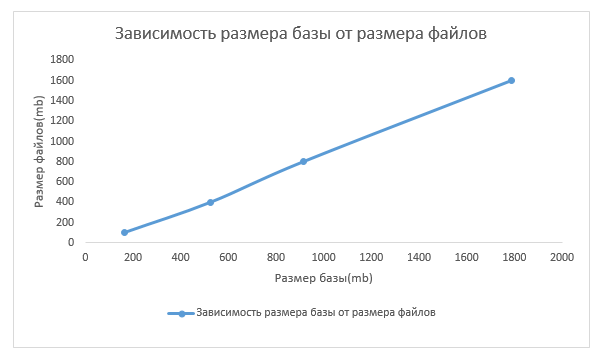
\includegraphics{sizeF_sizeB.png}

Зависимость тоже близка к линейной.

В итоге я измерил время работы программы пытаясь найти 100мб образцов в базах разных размеров (которые были получены ранее).

\begin{itemize}
	\item 162mb -- 0m17.022s
	\item 525mb -- 0m17.868s
	\item 915mb -- 0m19.057s
	\item 1789mb -- 0m20.725s
\end{itemize}

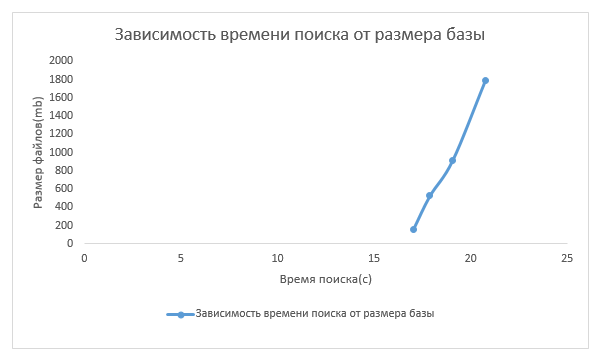
\includegraphics{sizeB_time.png}

Отсюда можно увидеть, что основное время тратиться на процесс создания "отпечатка"\, песни, чем на сам поиск. И поэтому если заранее создать большую базу "отпечатков"\,, то поиск можно осуществлять достаточно быстро.
\pagebreak
